\section{Bil}

\subsection{Diagrammer for bil}

\subsubsection{BDD for bil} % bdd_bil.pdf

Dette diagram viser blokken bil fra figur \ref{fig:bdd_au2}. Blokken 'bil' skal forstås som alle mekaniske og elektriske moduler som er fastgjort på køretøjet. Således er 

\begin{figure}[h]
\centering
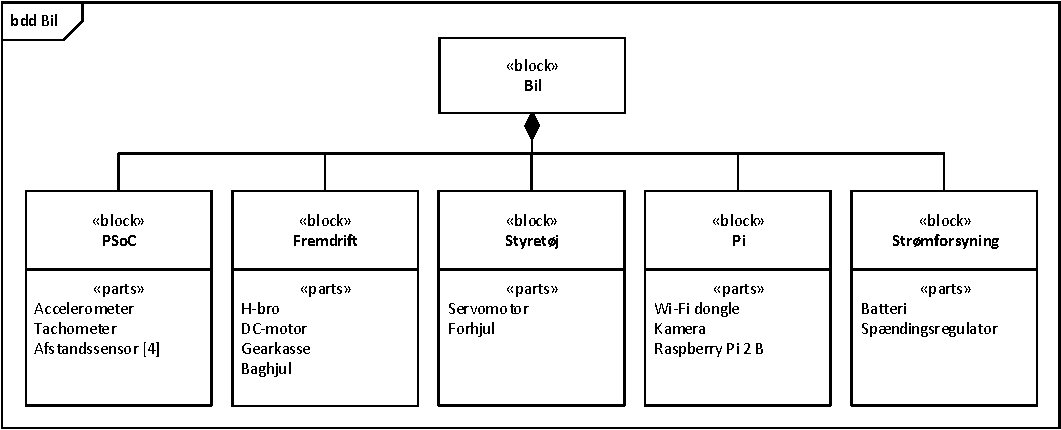
\includegraphics[width=\textwidth]{../fig/diagrammer/bil/bdd_bil.pdf}
\caption{BDD for bil}
\label{fig:bdd_bil}
\end{figure}
\clearpage

\subsubsection{IBD for signaler i bil}

På figur \ref{fig:ibd_bil} ses de interne forbindelser for figur \ref{fig:bdd_bil}. Diagrammet skaber et overblik over hvilke signaler der sendes og modtages. Bemærk at forsyningerne ikke er medtaget på diagrammet, istedet er disse vist i et selvstændigt diagram. Forsyningerne kan ses på figur \ref{fig:ibd_bil_forsyning}.

\begin{figure}[h]
\centering
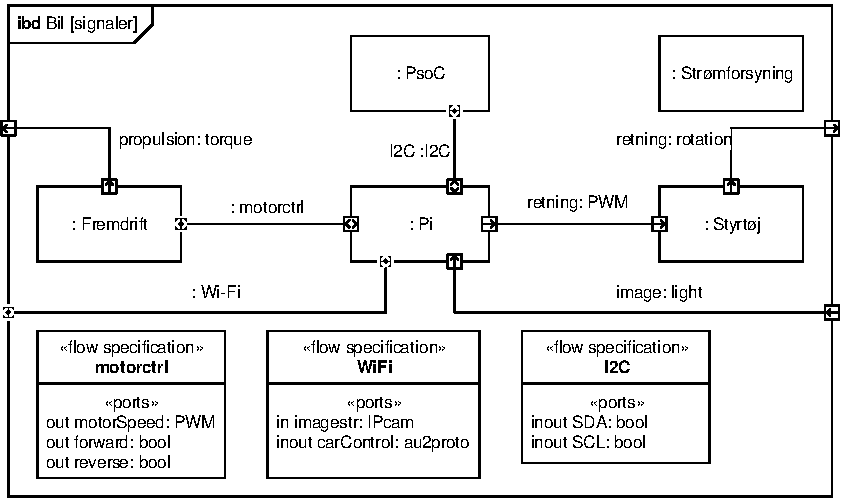
\includegraphics[scale=1]{../fig/diagrammer/bil/ibd_bil.pdf}
\caption{IBD for bil}
\label{fig:ibd_bil}
\end{figure}

\clearpage
\subsubsection{Signalbeskrivelser for bilens signaler}

\begin{table}[h]
	\centering
	\begin{tabularx}{\textwidth}{|l|Z|Z|Z|} \hline
	\textbf{Signal (navn: type)} & \textbf{Funktion} & \textbf{Tolerancer} & \textbf{Kommentarer} \\ \hline

Propulsion: torque
	& Baghjulenes torque til underlaget.
	& ~
	& ~
	\\ \hline

motorSpeed: PWM
	& Et PWM signal der bestemmer motorhastigheden. 
	& Frekvens: 30kHz +/- 1kHz 0-5V +/- 0.2V
 	& Logisk signal: \newline
		Lav = 0V +/- 0.2V \newline
		Høj = 5V +/- 0.2V
	\\ \hline

forward: bool
	& Kontrolsignal til H-bro.
	& 0-5V $\pm$ 0.2V
	& Lav = 0V +/- 0.2V  ’idle’ \newline
		Høj =  5V +/- 0.2V  ’frem’
	\\ \hline
	
reverse: bool
	& Kontrolsignal til H-bro.
	& 0-5V $\pm$ 0.2V
	& Lav = 0V +/- 0.2V ’idle’ \newline
		Høj =  5V +/- 0.2V  ’tilbage’
	\\ \hline
	
Inout SDA: bool
	& \IIC dataline til sensorer herunder accelerometer og afstandssensorer. 
	& 0-5V $\pm$ 0.5V
 	& Logisk signal: \newline
		Lav = 0V $\pm$ 0.5V \newline
		Høj = 5V $\pm$ 0.5V
	\\ \hline

Inout SCL: bool
	& \IIC clockline  til sensorer herunder accelerometer og afstandssensorer. 
	& 0-5V $\pm$ 0.5V
 	& Logisk signal: \newline
		Lav = 0V $\pm$ 0.5V \newline
		Høj = 5V $\pm$ 0.5V
	\\ \hline

Pulses: sound
	& Ultralydsbølger afsendt af sensor. 
	& Jfv. Datablad (henvisning kommer senere) %TODO henvsining
 	& ~
	\\ \hline
	
reflection: sound
	& Refleksionsbølge af udsendte ultralydsbølger. 
	& Jfv. Datablad (henvisning kommer senere) %TODO henvsining
 	& ~
	\\ \hline
	
retning: PWM 
	& PWM signal der vha pulsbredden angiver hvilken retning servomotoren skal 				dreje og dermed hvilken retning bilen skal dreje. 
	& Pulsbredde: 0.5ms – 2.5ms \newline
		Freq = 360Hz \newline
		0.5ms = 18\% Duty cycle (Venstre)\newline
		2.5ms = 90\% Duty cycle (Højre)
	& ~
	\\ \hline

retning: rotation
	& Får bilen til at dreje.
	& 30 grader til hhv. venstre og højre $\pm$ 5 grader
	& ~
	\\ \hline
	
imagestr: IPcam
	& At streame video fra bilens påmonterede kamera.
	& \textit{Ikke angivet} 
	& Laves med 3.parts software.
	\\ \hline

carControl: au2proto
	& At give styreinput fra brugeren til bilen.
	& \textit{Ikke angivet} 
	& Socketforbindelse.
	\\ \hline

	\end{tabularx}
	\label{tbl:bil_signaler}
\end{table}

\clearpage

\subsubsection{Forsyninger} % ibd_bil_forsyning.pdf

Diagrammet på figur \ref{fig:ibd_bil_forsyning} tilsvarer direkte figur \ref{fig:ibd_bil}, blot med beskrivelsen af forsyning. Dette giver forbedret overblik da de to diagrammer sat sammen bliver uoverskueligt.  

\begin{figure}[h]
\centering
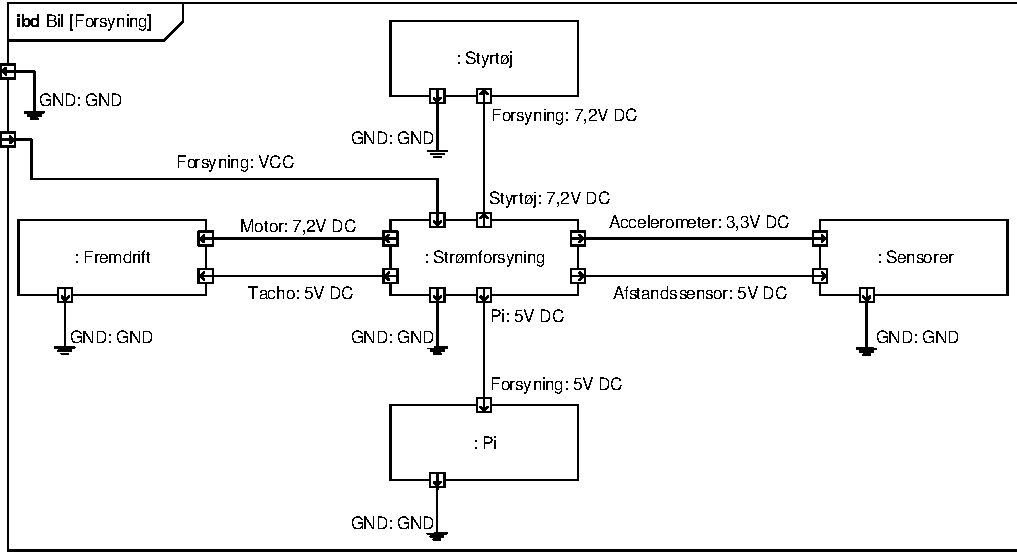
\includegraphics[width=\textwidth]{../fig/diagrammer/bil/ibd_bil_forsyning.pdf}
\caption{IBD for bilens forsyninger}
\label{fig:ibd_bil_forsyning}
\end{figure}

\clearpage

\subsubsection{Signalbeskrivelse for bilens forsyning}

\begin{table}[h]
	\centering
	\begin{tabularx}{\textwidth}{|l|Z|Z|Z|} \hline
	\textbf{Signal (navn: type)} & \textbf{Funktion} & \textbf{Tolerancer} & \textbf{Kommentarer} \\ \hline
forsyning: VCC
	& Forsyningsspænding fra det tilkoblede batteri. 
	& 7.2V DC $\pm$ 1V max. 20A
 	& Aflæst på batteriet.
	\\ \hline
	
GND: GND
	& Reference. 
	& 0V
 	& ~
	\\ \hline
	
styretøj: 5V DC
	& Forsyningsspænding til styrtøj herunder servomotor. 
	& 5V DC $\pm$ 0,5V max 400 mA
 	& Fundet i databladet for servoen \cite{lib:servo}.
	\\ \hline
	
PSoC: 5V DC
	& Forsyningsspænding til PSoC. 
	& 5V DC $\pm$ 0,5V max 500 mA
 	& Worst case vurdering på baggrund af USB forsyning fra PC.
	\\ \hline
	
	
accelerometer: 3.3V DC
	& Forsyningsspænding til accelerometeret.
	& 3.3V DC $\pm$ 0.2V max 8 mA
 	& Fundet i databladet for servoen \cite{lib:accel}.
	\\ \hline
	
afstandssensor: 5V DC
	& Individuel forsyningsspænding til afstandssensorerne.
	& 5V DC $\pm$ 0.5V max 400 mA
 	& Fundet i databladet for sensorerne \cite{lib:maxsonar}.
	\\ \hline
	
Pi: 5V DC
	& Individuel forsyningsspænding til Pi.
	& 5V DC $\pm$ 0.5V max 1.8A
 	& Aflæst i FAQ for Pi \cite{lib:PI2PSU}.
	\\ \hline
	
Tachomet: 5V DC
	& Individuel forsyningsspænding til tachometeret.
	& 5V DC $\pm$ 0.5V max 8 mA
 	& Aflæst i datablad for sensor \cite{lib:tacho}.
	\\ \hline
	
motor: 7.2V DC
	& Individuel forsyningsspænding til motoren.
	& 7.2V DC $\pm$ 1V max 2A

 	& Udregnet ud fra stall-test i laboratoriet.
	\\ \hline
	\end{tabularx}
	\label{tbl:bil_forsyninger}
\end{table}
\clearpage
\subsection{Fremdrift}

Bilens fremdrift forårsages af motoren samt tilhørende elektronik, hvilket er beskrevet på figur \ref{fig:ibd_fremdrift}. Det skal igen noteres at forsyningen til H-broen ikke er medtaget på diagrammet, men findes på figur \ref{fig:ibd_bil_forsyning}. Motoren trækker altså ikke sin strøm fra signalet motorCtrl. 

\begin{figure}[h]
\centering
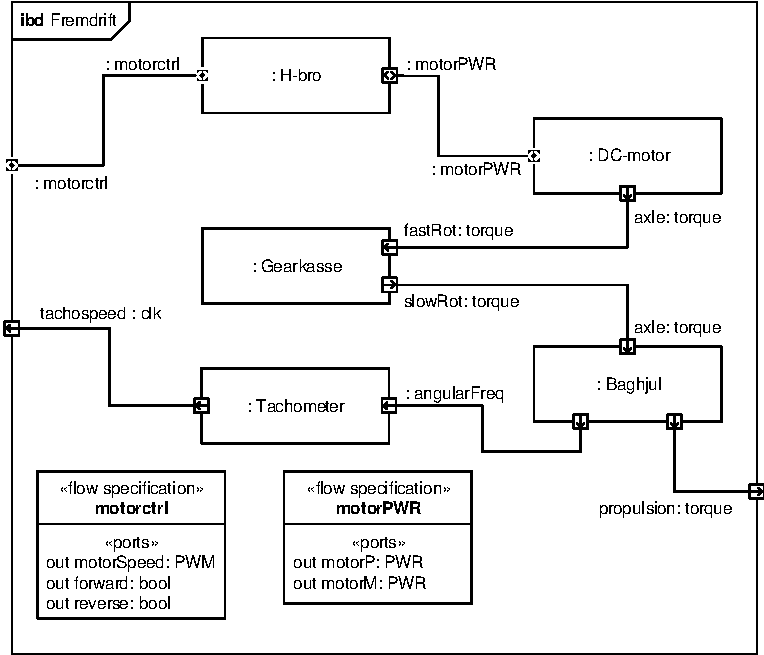
\includegraphics[scale=1]{../fig/diagrammer/bil/ibd_fremdrift.pdf}
\caption{IBD for blokken fremdrift}
\label{fig:ibd_fremdrift}
\end{figure}

\clearpage

\subsubsection{Signalbeskrivelse for fremdrift}

\begin{table}[h]
	\centering
	\begin{tabularx}{\textwidth}{|l|X|X|X|} \hline
	\textbf{Signal (navn: type)} & \textbf{Funktion} & \textbf{Tolerancer} & \textbf{Kommentarer} \\ \hline
motorSpeed: PWM
	& Et PWM signal der bestemmer motorhastigheden. 
	& Frekvens: 30kHz +/- 1kHz 0-5V +/- 0.2V
 	& Logisk signal: \newline
		Lav = 0V +/- 0.2V \newline
		Høj = 5V +/- 0.2V
	\\ \hline

forward: bool
	& Kontrolsignal til H-bro.
	& 0-5V $\pm$ 0.2V
	& Lav = 0V +/- 0.2V  ’idle’ \newline
		Høj =  5V +/- 0.2V  ’frem’
	\\ \hline
	
reverse: bool
	& Kontrolsignal til H-bro.
	& 0-5V $\pm$ 0.2V
	& Lav = 0V +/- 0.2V ’idle’ \newline
		Høj =  5V +/- 0.2V  ’tilbage’
	\\ \hline
	
motorP: PWR
	& Et PWM med frekvens som motorSpeed, dog med mulighed for højere effekt. Dette signal forsyner motoren.
	& Frekvens: 30kHz +/- 1kHz 0-7,2V +/- 0.5V

 	& Logisk signal: \newline
		Lav = 0V +/- 0.5V \newline 
		Høj = 7,2V +/- 0.5V
	\\ \hline

motorM: PWR
	& Reference til motorP.
	& 0V $\pm$ 0.5V
	& ~
	\\ \hline
	
fastRot: torque
	& Kraft der overføres fra motor til gearkasse via drivaksel.
	& - 
	& ~
	\\ \hline
	
slowRot: torque
	& Kraft der overføres fra gearkasse til baghjul via drivaksel.
	& - 
	& ~
	\\ \hline
	
: angularFreq
	& Hjulenes omdrejningshastighed.
	& - 
	& ~
	\\ \hline
	
tachoSpeed: freq
	& Digitalt signal med varierende frekvens afhængig af baghjulenes 					omdrejningshastighed.
	& - 
	& Vejledende: \newline
		64Hz = 10Km/t \newline
		Logisk signal: \newline
		Lav = 0V +/- 0.2V \newline
		Høj = 5V +/- 0.2V

	\\ \hline
	
Propulsion: torque
	& Baghjulenes torque til underlaget.
	& - 
	& ~
	\\ \hline
	\end{tabularx}
\end{table}
\clearpage
\subsection{Styretøj}

De interne signaler for blokken styretøj er beskrevet nedenfor i figur \ref{fig:ibd_styretoej}.

\begin{figure}[h]
\centering
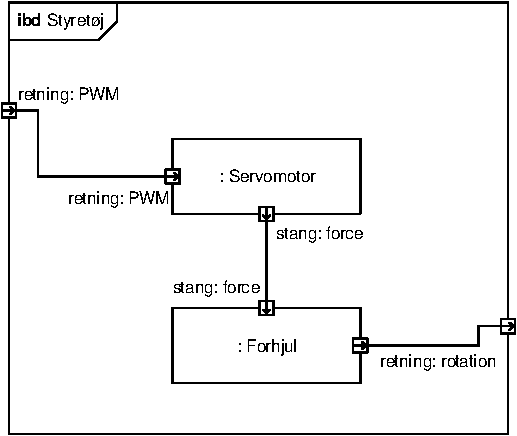
\includegraphics[scale=1]{../fig/diagrammer/bil/ibd_styretoej.pdf}
\caption{IBD for blokken styretøj}
\label{fig:ibd_styretoej}
\end{figure}

\subsubsection{signalbeskrivelse for styretøj}

\begin{table}[h]
	\centering
	\begin{tabularx}{\textwidth}{|l|Z|Z|Z|} \hline
	\textbf{Signal (navn: type)} & \textbf{Funktion} & \textbf{Tolerancer} & \textbf{Kommentarer} \\ \hline
retning: PWM 
	& PWM signal der vha pulsbredden angiver hvilken retning servomotoren skal dreje og dermed hvilken retning bilen skal dreje. 
	& Pulsbredde: 0.5ms – 2.5ms \newline
		Freq = 360Hz \newline
		0.5ms = 18\% Duty cycle (Venstre)\newline
		2.5ms = 90\% Duty cycle (Højre)
	& ~
	\\ \hline
stang: force 
	& Skal overføre kraften fra servomotoren til forhjulene. Dette sker via en stang.
	& -
	& ~
	\\ \hline
retning: rotation
	& Får bilen til at dreje.
	& 30 grader til hhv. venstre og højre $\pm$ 5 grader
	& ~
	\\ \hline
	\end{tabularx}
\end{table}
\clearpage
\subsection{Pi}

Her beskrives intern kommunikation for controlleren Pi i systemet. 

\begin{figure}[h]
\centering
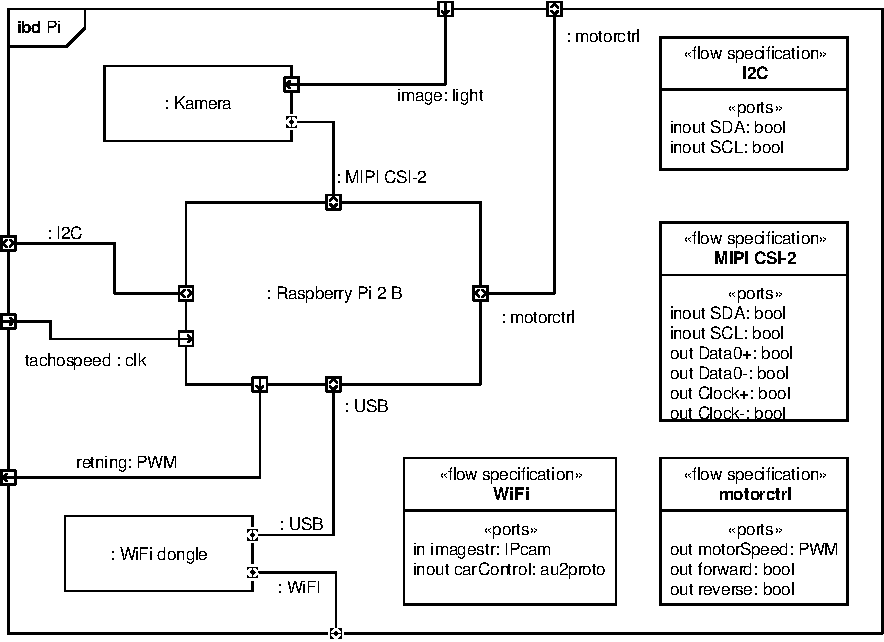
\includegraphics[scale=1]{../fig/diagrammer/bil/ibd_pi.pdf}
\caption{IBD for blokken Pi}
\label{fig:ibd_pi}
\end{figure}
\clearpage


\subsubsection{Signalbeskrivelse for Pi}

\begin{table}[h]
	\centering
	\begin{tabularx}{\textwidth}{|l|Z|Z|Z|} \hline
	\textbf{Signal (navn: type)} & \textbf{Funktion} & \textbf{Tolerancer} & \textbf{Kommentarer} \\ \hline
SDA: bool
	& I2C dataline til sensorer herunder accelerometer og afstandssensorer  
	& 0-5V$\pm$0.5V 
 	& Logisk signal: 			\newline
		Lav= 0V$\pm$0.5V  	\newline
		Høj= 7.2V$\pm$0.5V
	\\ \hline
	
SCL: bool
	& I2C clockline  til sensorer herunder accelerometer og afstandssensorer
	& 0-5V$\pm$0.5V
	& Logisk signal:			\newline 
		Lav= 0V$\pm$0.5V 	\newline
		Høj= 7.2V$\pm$0.5V
	\\ \hline
	
Image: light
	& Lysindfald til kamerasensor
	& -
	& -
	\\ \hline

motorSpeed: PWM	
	& Et PWM signal der bestemmer motorhastigheden.	
	& Frekvens: 30kHz$\pm$1kHz \newline
	  0-5V$\pm$0.2V	
	& Logisk signal: 			\newline 
		Lav= 0V$\pm$0.2V 	\newline
		Høj= 5V$\pm$0.2V
	\\ \hline
	
forward: bool	
	& Kontrolsignal til H-bro
	& 0-5V$\pm$0.2V
	& Logisk signal:					\newline 
		Lav= 0V$\pm$0.2V  ''idle''		\newline
		Høj= 5V$\pm$0.2V  ''forward''
	\\ \hline
	
reverse: bool	
	& Kontrolsignal til H-bro
	& 0-5V$\pm$0.2V	
	& Logisk signal: 					\newline
		Lav= 0V$\pm$0.2V ''idle''		\newline
		Høj= 5V$\pm$0.2V ''back''
	\\ \hline
	
:USB 	
	& Serielforbindelse mellem Wi-fi dongle og Pi	
	& VBUS = 5V$\pm$0.2V 				\newline 
	  D$-$ = 5V$\pm$0.2V				\newline
	  D$+$ = 5V$\pm$0.2V				\newline
	  GND = 0V							\newline	  
	  & VBUS for Low-power port: 		\newline
		Diff  ''1''						\newline
		(D$+$)-(D$-$) > 200 mV			\newline
		og D$+$>VIH (min)				\newline

		Diff ''0''						\newline
		(D$-$)-(D$+$) > 200 mV			\newline
		og D$-$>VIH (min)				\newline
	\\ \hline	
	
imagestr: IPcam
	& At streame video fra kameraet påmonteret på bilen til PC'en.
	& \textit{Ikke angivet} 
	& Laves med 3. parts software	
	\\ \hline

carControl: au2proto
	& At sende data til og fra PC'en til bilen.
	& \textit{Ikke angivet} 
	& ~
	\\ \hline
	
: MIPI CSI-2
	& Kamera serielt interface
	& \textit{Ikke angivet} 
	& Se reference: \cite{lib:MIPICSI-2}
	\\ \hline
	\end{tabularx}
\end{table}

\clearpage
\subsection{PSoC}

På figur \ref{fig:ibd_psoc} ses de interne signaler for blokken PSoC.

\begin{figure}[h]
\centering
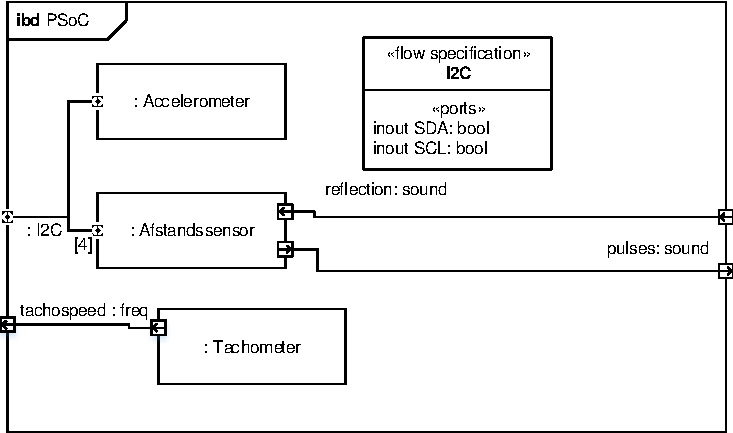
\includegraphics[scale=1]{../fig/diagrammer/bil/ibd_PSoC.pdf}
\caption{IBD for blokken PSoC}
\label{fig:ibd_psoc}
\end{figure}

\subsubsection{Signalbeskrivelse for PSoC}

\begin{table}[h]
	\centering
	\begin{tabularx}{\textwidth}{|l|Z|Z|Z|} \hline
	\textbf{Signal (navn: type)} & \textbf{Funktion} & \textbf{Tolerancer} & \textbf{Kommentarer} \\ \hline
Inout SDA: bool
	& \IIC dataline til sensorer herunder accelerometer og afstandssensorer. 
	& 0-5V $\pm$ 0.5V
 	& Logisk signal: \newline
		Lav = 0V $\pm$ 0.5V \newline
		Høj = 5V $\pm$ 0.5V
	\\ \hline

Inout SCL: bool
	& \IIC clockline  til sensorer herunder accelerometer og afstandssensorer. 
	& 0-5V $\pm$ 0.5V
 	& Logisk signal: \newline
		Lav = 0V $\pm$ 0.5V \newline
		Høj = 5V $\pm$ 0.5V
	\\ \hline

Pulses: sound
	& lydbølger afsendt af sensor. 
	& Ultralydsfrekvens på 42kHz
 	& ~
	\\ \hline
	
reflections: sound
	& Refleksionsbølge fra forhindring. 
	& delay'ed Ultralydsfrekvens på 42kHz
 	& ~
	\\ \hline
	
tachoSpeed: freq
	& Digitalt signal med varierende frekvens afhængig af baghjulenes omdrejningshastighed.
	& ~
	& Vejledende: \newline
		64Hz = 10Km/t \newline
		Logisk signal: \newline
		Lav = 0V +/- 0.2V \newline
		Høj = 5V +/- 0.2V	\\ \hline
	\end{tabularx}
\end{table}
\clearpage
\subsection{MPU-6050 Accelerometer/Gyroskop}

MPU-6050 er en kombination af et accelerometer, et gyroskop, begge med 3 akser og et termometer. Det betyder for systemet at det er i stand til at registrere en ændring i acceleration og/eller orientering i alle retninger. Sensoren er blevet valgt til projektet på baggrund af et \IIC interface, som derved kan tilkobles en samlet bus sammen med andre sensorer på bilen. Udover dette giver det konstruerede breakoutboard mulighed for nem tilslutning, men fortsat lille størrelse på sensoren.
Sensoren fungerer altid som en slave med adressen $0b110100X$, hvor X bliver bestemt af det logiske niveau på pin AD0, der som standard er lav. 

\begin{figure}[h]
	\centering
	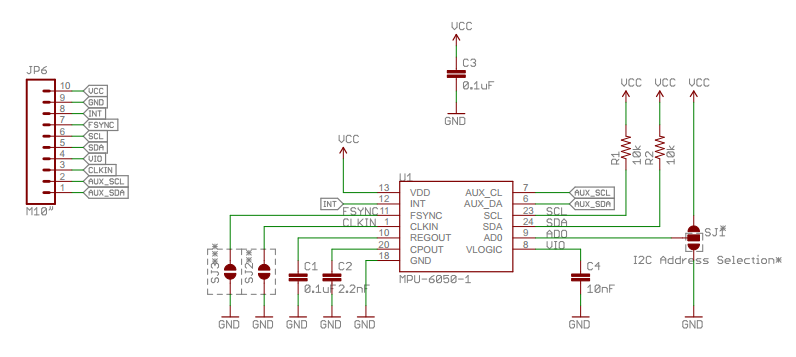
\includegraphics[scale=0.7]{../fig/billeder/mpu6050.png}
	\caption{MPU-6050 diagram}
	\label{fig:mpu6050}
\end{figure}

Diagrammet for sensoren er vist i figur \ref{fig:mpu6050}. Maksimal bushastighed for MPU-6050 er 400kHz, men da der er andre sensorer som arbejder langsommere end MPU-6050 i systemet, passer den fint ind. Accelerometeret er en MEMS-type, hvor der er bygget mikroskopiske kondensatorer ind i chippen, som kan fjedre og bevæge sig, hvilket registreres som en ændring i kapacitans. Denne ændring kan omregnes til nogle brugbare værdier, og kan herfra anvendes til bl.a. retningsbestemmelse. Der er i alt 7 16-bits registre i sensoren, som hver især er tilknyttet til en ADC på hver akse, med undtagelse af register nr. 7, som er tilknyttet termometeret. 
Protokollen for kommunikation med sensoren ser således ud:

\begin{figure}[h]
	\centering
	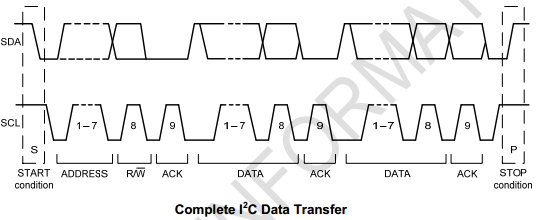
\includegraphics[scale=0.8]{../fig/billeder/mpu6050i2c.png}
	\caption{\IIC protokol for MPU-6050}
	\label{fig:mpu6050i2c}
\end{figure}

Som det ses i figur \ref{fig:mpu6050i2c}, starter masteren med at sætte en startsekvens ud på SDA (HIGH-to-LOW), mens SCL er høj. Herefter betragtes bussen som optaget, indtil der bliver sendt en stopsekvens på SDA (LOW-to-HIGH) af masteren, mens SCL ligeledes er høj. Efter startsekvensen bliver der sendt en 7-bits adresse og en R/W bit. Data der bliver transmitteret over \IIC bliver sendt i pakker af 8 bits. Når der først er sendt en startsekvens, er der ingen begrænsning på hvor meget data der må sendes, udover at der efter hver pakke, skal registreres en acknowledge. MPU-6050 indeholder desuden en DMP (Digital Motion Processor), som har til opgave at håndtere noget af dataprocesseringen fra selve MPU-6050. 
